\documentclass[tikz, border=7pt]{standalone}
\usepackage{tikz}


\begin{document}
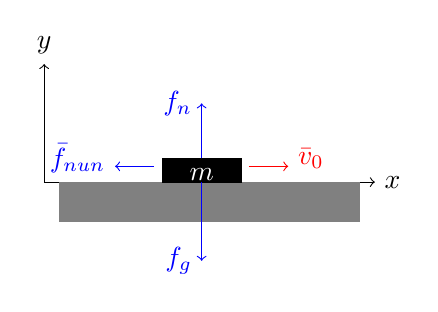
\begin{tikzpicture}
% hnitakerfi
\draw [<->] (0,1.5) -- (0,0) -- (4.2,0);
\node [above] at (0,1 .5) {$y$};
\node [right] at (4.2,0) {$x$};
\draw [fill=gray, gray] (0.2,-0.5) rectangle (4,0);
% pökkur
\draw [fill=black] (1.5,0) rectangle (2.5,0.3);
\node [white] at (2,0.1) {$m$};
% vigrar
\draw [red, ->] (2.6,0.2) -- (3.1,0.2);
\node [red, right] at (3.1,0.3) {$\bar{v}_0$};
\draw [blue, <-] (0.9,0.2) -- (1.4,0.2);
\node [blue, left] at (0.9,0.3) {$\bar{f}_{nun}$};

%þyngdar- normalkraftur
\draw [blue, ->] (2,0) -- (2,-1) node [left] {$f_g$};
\draw [blue, ->] (2,0.3) -- (2,1) node [left] {$f_n$};

\end{tikzpicture}
\end{document}
